\documentclass{article} 
\UseRawInputEncoding
\usepackage[utf8]{inputenc}
\usepackage[T1]{fontenc}
\usepackage{selinput}
\usepackage[spanish]{babel}
\usepackage{hyphenat}
\usepackage{graphicx} 
\usepackage{subcaption}
\usepackage{hyperref}
\usepackage{listings}
\usepackage{xcolor}
\usepackage{float}
\SelectInputMappings{%
  eacute={é},
}

\definecolor{codegreen}{rgb}{0,0.6,0}
\definecolor{codegray}{rgb}{0.5,0.5,0.5}
\definecolor{codepurple}{rgb}{0.58,0,0.82}
\definecolor{backcolour}{rgb}{0.95,0.95,0.92}

\lstdefinestyle{mystyle}{
    backgroundcolor=\color{backcolour},
    commentstyle=\color{codegreen},
    keywordstyle=\color{blue},
    numberstyle=\tiny\color{codegray},
    stringstyle=\color{codepurple},
    basicstyle=\ttfamily\footnotesize,
    breakatwhitespace=false,
    breaklines=true,
    captionpos=b,
    keepspaces=true,
    numbers=left,
    numbersep=5pt,
    showspaces=false,
    showstringspaces=false,
    showtabs=false,
    tabsize=2
}

\lstdefinelanguage{CSS}{
  keywords={color,background-image:,margin,padding,font,weight,display,position,top,left,right,bottom,list,style,border,size,white,space,min,width, transition:, transform:, transition-property, transition-duration, transition-timing-function},	
  sensitive=true,
  morecomment=[l]{//},
  morecomment=[s]{/*}{*/},
  morestring=[b]',
  morestring=[b]",
  alsoletter={:},
  alsodigit={-}
}
\lstset{style=mystyle}
\date{} 

\begin{document} 

\begin{center}
    
\includegraphics[width=1\textwidth]{Images/Imagenes/logo/LogoBIASbn.png}\\ 
\end{center}
    
\title{BIAS} 

\vspace{1cm} 

\textbf{Integrantes del Proyecto:} 

\begin{itemize}
    \item Adell, Nicolas Fabian
    \item De Blasi, Luca
    \item Diaz Melion, Danilo Sebastian
    \item Gil Soria, Ian Lucas
    \item Montenegro, Luciano Nahuel
    \item Sojka, Santiago Alejandro
\end{itemize}

\tableofcontents 

\newpage 

\section{Introducción}

BIAS es un módulo aplicable a una silla de ruedas que permite a los usuarios dirigirla mediante el sus pensamientos, eliminando la necesidad de controles físicos tradicionales y optimizando la experiencia de movilidad. Este proyecto representa un avance significativo en el campo de la movilidad asistida, con el objetivo de mejorar la independencia y la calidad de vida de las personas con movilidad reducida.

Este sistema se basa en la avanzada tecnología de interfaz cerebro-computadora (BCI), la cual captura las señales neuronales del usuario y las traduce en comandos precisos para maniobrar la silla de ruedas sin esfuerzo. Además, el diseño modular y adaptable del sistema permite su integración en diversos modelos de sillas de ruedas y su personalización según las necesidades específicas de cada usuario. 

La seguridad es una prioridad fundamental en este desarrollo, por lo que el módulo incorpora múltiples capas de redundancia y verificación de señales, asegurando que la silla de ruedas responda de manera precisa y confiable a las intenciones del usuario. 

Aspiramos a revolucionar la forma en que las personas con movilidad reducida interactúan con su entorno, brindándoles una herramienta que amplía su capacidad para controlar su vida de manera más segura e independiente.

\subsection{Resumen del proyecto}
Este proyecto se centra en el desarrollo de una silla de ruedas controlada mediante señales cerebrales. El sistema se compone principalmente de los siguientes componentes: la silla de ruedas, un dispositivo EEG (electroencefalograma) y dos motores que permiten al usuario moverse en la dirección deseada.

El funcionamiento del sistema es el siguiente: el usuario se sienta en la silla y se coloca el EEG en la cabeza. A continuación, el usuario piensa en la dirección en la que desea moverse, y los motores responden en consecuencia.

El EEG tiene la función de leer las señales cerebrales del usuario. Estas señales se clasifican en las categorías de alpha, beta, gamma, delta y theta, y luego se someten a un proceso de filtrado para eliminar cualquier ruido. Posteriormente, las señales filtradas son analizadas por una Inteligencia Artificial (IA) desarrollada por nuestro equipo, la cual identifica patrones para determinar si el usuario desea moverse o detenerse.

Además, la silla está equipada con un sistema de emergencia que se activa en caso de lecturas erróneas o la detección de obstáculos. Este sistema de emergencia está compuesto por sensores infrarrojos y ultrasónicos que detectan la presencia de obstáculos frente a la silla.

\subsection{Motivación}
Como estudiantes de séptimo año, buscamos desarrollar un proyecto con el fin de cumplir con el requerimiento horario de practicas profesionalizantes. Nuestra intención inicial fue encontrar el proyecto ideal en cuestiones de impacto social, enfocándonos en la mejora de la calidad de vida de aquellas personas con discapacidades. Bajo este marco, y tras una extensa investigación, proponemos crear un módulo aplicable a una silla de ruedas controlado mediante la actividad cerebral del usuario, utilizando tecnología de interfaces cerebro-computadora (BCI), para brindarles mayor autonomía, independencia y participación social.   Creemos que este proyecto tiene el potencial de transformar la vida de las personas con movilidad motora reducida debido a enfermedades como ELA, esclerosis múltiple o cuadriplejia, permitiéndoles controlar su propio movimiento y mejorar significativamente su calidad de vida.
\subsection{Objetivos}
El objetivo de este proyecto es desarrollar una silla de ruedas motorizada que pueda ser controlada por la actividad cerebral del usuario. Esto beneficiaría a las personas con discapacidades motoras severas para lograr independencia y movilidad, mejorando su calidad de vida y participación en la sociedad. De esta manera, estas personas las cuales no pueden caminar o tienen movilidad reducida, pueden gozar de la utilización de una silla de ruedas controlada por señales cerebrales sin la utilización de ambas manos y meramente por sus pensamientos, dándole libertad y autonomía al usuario.

\section{¿Quiénes somos?}
Somos el grupo BIAS (Brain Intelligence Artificial System), conformado por seis estudiantes de la especialidad de Aviónica del séptimo año, segunda división, comisión C, de la Escuela Técnica N° 7 IMPA "Taller Regional Quilmes". Nuestro equipo se encuentra comprometido en el desarrollo de un módulo adaptable para sillas de ruedas, para así poder brindarles mas independencia y movilidad.
\subsection{Contactos}

En este apartado se detallarán los contactos a los integrantes del proyecto, adjuntando enlaces a sus redes:

\subsubsection{Adell Nicolás}

    \href{https://instagram.com/nicolas.adell}{Instagram}

    
    \href{http://www.linkedin.com/in/nicolas-adell-354508297}{LinkedIn}

    
    \href{mailto:nicolas.fabian2005@gmail.com}{Gmail}

\subsubsection{De Blasi Luca}

    \href{https://instagram.com/luca.deblasii}{Instagram}

    
    \href{https://www.linkedin.com/in/luca-de-blasi-31164b304}{LinkedIn}

    
    \href{mailto:luqac2006@gmail.com}{Gmail}

\subsubsection{Diaz Melión Danilo}

    \href{https://instagram.com/_danilodiaz}{Instagram}

    
    \href{https://www.linkedin.com/in/danilodiazmelion/}{LinkedIn}

    
    \href{mailto:danilodiaz934@gmail.com}{Gmail}

\subsubsection{Gil Soria Ian}

    \href{https://instagram.com/ian_gilsooor}{Instagram}

    
    \href{https://www.linkedin.com/in/ian-lucas-gil-soria-a8090b2a8?utm_source=share&utm_campaign=share_via&utm_content=profile&utm_medium=android_app}{LinkedIn}

    
    \href{mailto:ianlucasgilsoria@gmail.com}{Gmail}

\subsubsection{Montenegro Luciano}


    \href{https://instagram.com/luchito_.montenegro}{Instagram}

    
    \href{https://www.linkedin.com/in/luciano-montenegro-3215aa304}{LinkedIn}

    
    \href{mailto:lucianomontenegro1021@gmail.com}{Gmail}



\subsubsection{Sojka Santiago}

    \href{https://instagram.com/sojkaa.sant}{Instagram}

    
    \href{https://www.linkedin.com/in/santiago-sojka-817198271/}{LinkedIn}

    
    \href{mailto:santiagosojka@gmail.com}{Gmail}




\section{Desarrollo del Proyecto}
En este capítulo se expondrá en detalle la metodología empleada para avanzar en el desarrollo del proyecto, incluyendo las fuentes de inspiración y los proyectos similares que se tomaron como referencia para el diseño de nuestros circuitos y la programación de los sistemas. Además, se incluirán imágenes ilustrativas de estos proyectos de referencia, con el fin de ofrecer una comprensión visual más completa. Al finalizar el capítulo, se presentarán y explicarán los resultados obtenidos, evaluando su eficacia en relación con los objetivos planteados.

\subsection{Metodología}
La metodología aplicada en este proyecto se basa en la organización del equipo en dos grupos especializados. El primer grupo se encarga del desarrollo de los programas, siendo ejemplos de esto los filtros virtuales, programas de recepción y procesado, mientras que el segundo se dedica a la implementación de los motores, sistemas de emergencia y filtros. Esta división del trabajo permite una utilización más eficiente del tiempo, al abordar simultáneamente diversas áreas del proyecto, lo que resulta en un avance más significativo en periodos de tiempo más reducidos.


\subsection{Historia del Arte}
En este capitulo se repasa todos los conceptos previamente vistos mediante los cuales pudimos empezar a conceptualizar la idea del proyecto.



\subsubsection{Neuralink}
Uno de los casos que nos permitió aproximarnos a la conceptualización del proyecto fue el chip cerebral estilo implante de Neuralink, denominado Telepathy. Este dispositivo, desarrollado por la compañía de Elon Musk, tiene como objetivo facilitar la vida de las personas mediante la optimización de herramientas y su adaptación al cuerpo humano a través del implante. El chip crea una conexión entre el ser humano y dispositivos electrónicos, permitiendo, por ejemplo, controlar una puerta con traba eléctrica, desbloquear un teléfono móvil, e incluso monitorear el estado de ánimo de las personas.


Este ejemplo nos ofreció una perspectiva sobre la viabilidad de desarrollar un dispositivo, que, aunque no tan complejo, pudiera ser controlado por el propio cuerpo humano. A partir de esta premisa, iniciamos una investigación para explorar las posibilidades y opciones disponibles basadas en esta idea.


\subsubsection{Ryan Lopez EEG}
Si bien nuestro motivo y objetivo principal era crear un dispositivo original e innovador, también nos propusimos investigar proyectos con cierta similitud. En este proceso, encontramos el repositorio de un estudiante que desarrolló un sistema capaz de detectar señales alfa y, en función de las reacciones o pensamientos del usuario, permitir el control a través de un test de concentración. Este test consistía en que el usuario debía mantener un estado de concentración mientras estudiaba un documento para un examen, en lo que se podría considerar un simulacro.


El sistema desarrollado por Ryanlopezz activaba una alarma si los niveles de concentración del usuario comenzaban a disminuir, basándose en un espectro de señales alfa transmitidas por un conjunto de electrodos EEG dorados conectados a la cabeza del estudiante. Además, el sistema realizaba otras dos pruebas: una de ellas consistía en escribir en código Morse mediante pensamientos, enviando "pulsos de concentración", y la otra permitía controlar el movimiento de un personaje en el famoso videojuego "Flappy Bird", ajustando el impulso para subir o bajar.

En el siguiente link se adjunta la página de GitHub de Ryan Lopez en donde se puede observar más a detalle los programas y archivos de su EEG.


\begin{center}
    \href{https://github.com/ryanlopezzzz/EEG}{Ryan Lopez GitHub}
\end{center}


Gracias al mismo proyecto realizado por este usuario, pudimos desarrollar nuestro propio circuito para el sistema de filtrado, ya que íbamos a requerir otras especificaciones con diferentes funciones, tales como la entrada de señal: ya que esta debía ser mayor a la designada, al nosotros trabajar no solo con el espectro radioelectrico de las señales Alpha, sino con las principales señales que el cerebro produce al momento de realizar un pensamiento especifico; Por otro lado nosotros íbamos a requerir no solo un sistema de filtros EEG sino 4 placas del mismo circuito, debido a la posibilidad de maniobrar controlando los 3 ejes de los motores de la silla de ruedas


\begin{center}
    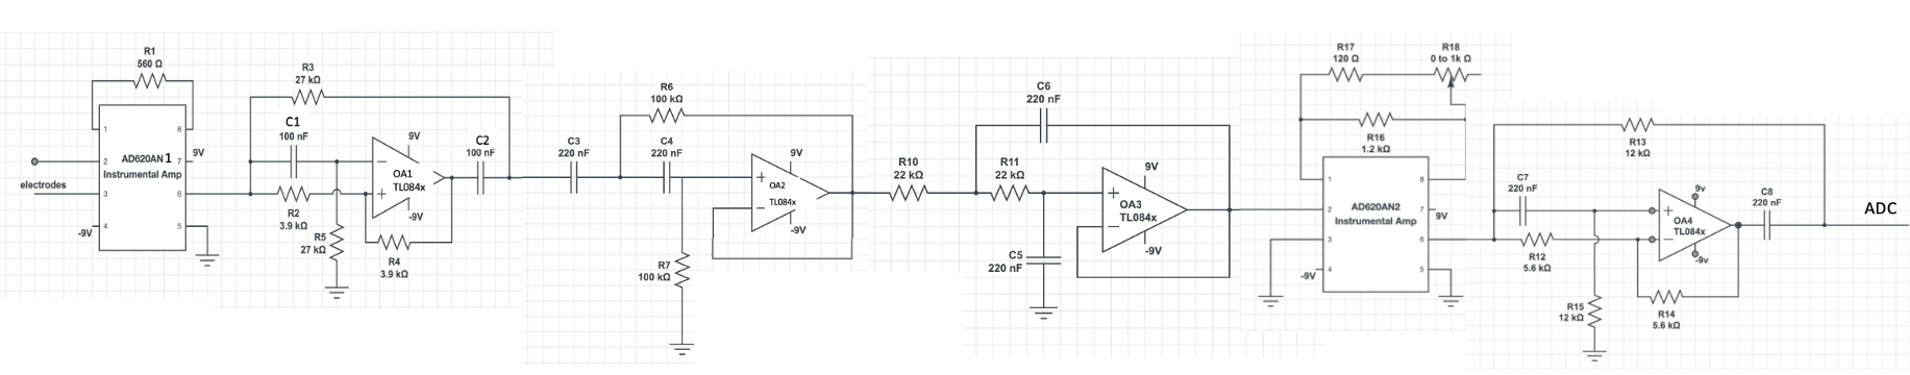
\includegraphics[width=1\textwidth]{Images/Imagenes/filtroeegderyan.png}\\
    
Por otro lado nos dio una primera vista de la localización de los botones EEG como irían colocados en la cabeza

\end{center}

\begin{center}
    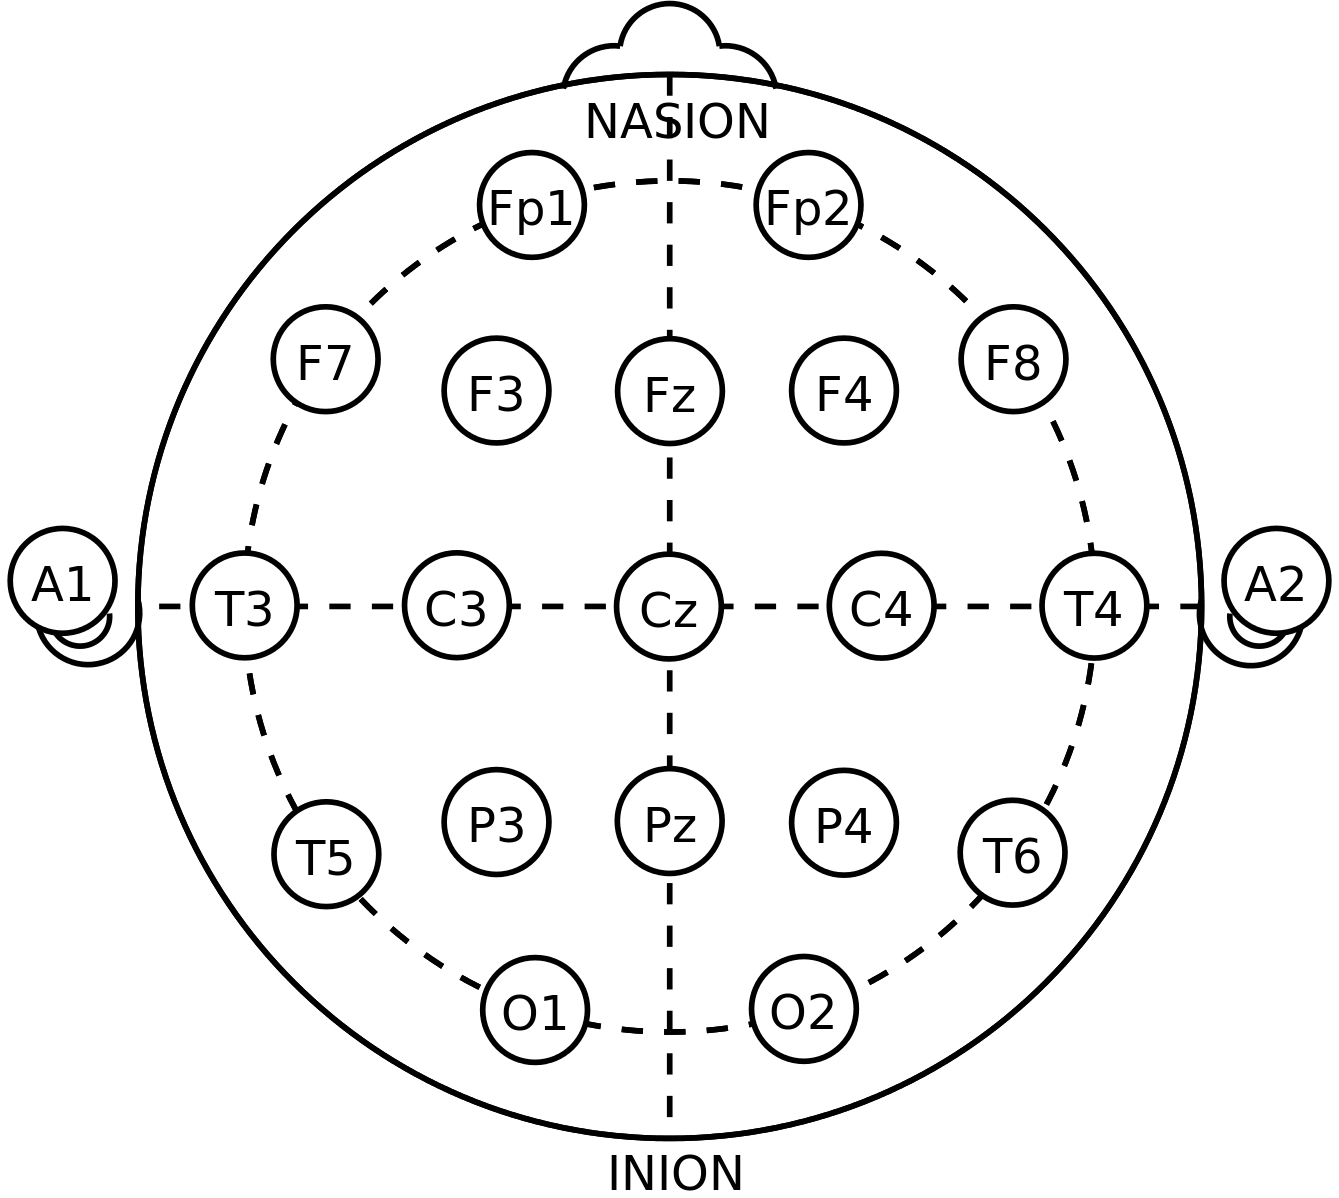
\includegraphics[width=1\textwidth]{Images/Imagenes/localizacionelectrodoseeg.png}\\

\end{center}

Así mismo para el estudio del aérea de medicina y saber como el cerebro humano se encarga de transmitir ciertas señales eléctricas gracias a la actividad cerebral  tuvimos en cuenta los actuales dispositivos de eneflografos, como se componen y actúan gracias ala actividad cerebral, bajo un especto radioelectrico determinado adjunto a la clasificación de las ondas transmitidas por el cerebro humano

\subsubsection{OpenBCI}

En nuestra búsqueda de conexiones para un microcontrolador y formas de desarrollar nuestro propio proyecto, descubrimos un sitio web llamado OpenBCI, una compañía especializada en la creación de dispositivos que integran tecnología con la interfaz del cuerpo humano. Esta empresa ha desarrollado un encefalógrafo casero, proporcionando dimensiones y parámetros estructurales que nos permitieron diseñar nuestra propia vincha/casco. Este dispositivo incorpora electrodos EEG, adaptados a la cabeza del usuario, como parte fundamental de nuestro proyecto "BIAS".

\begin{center}
    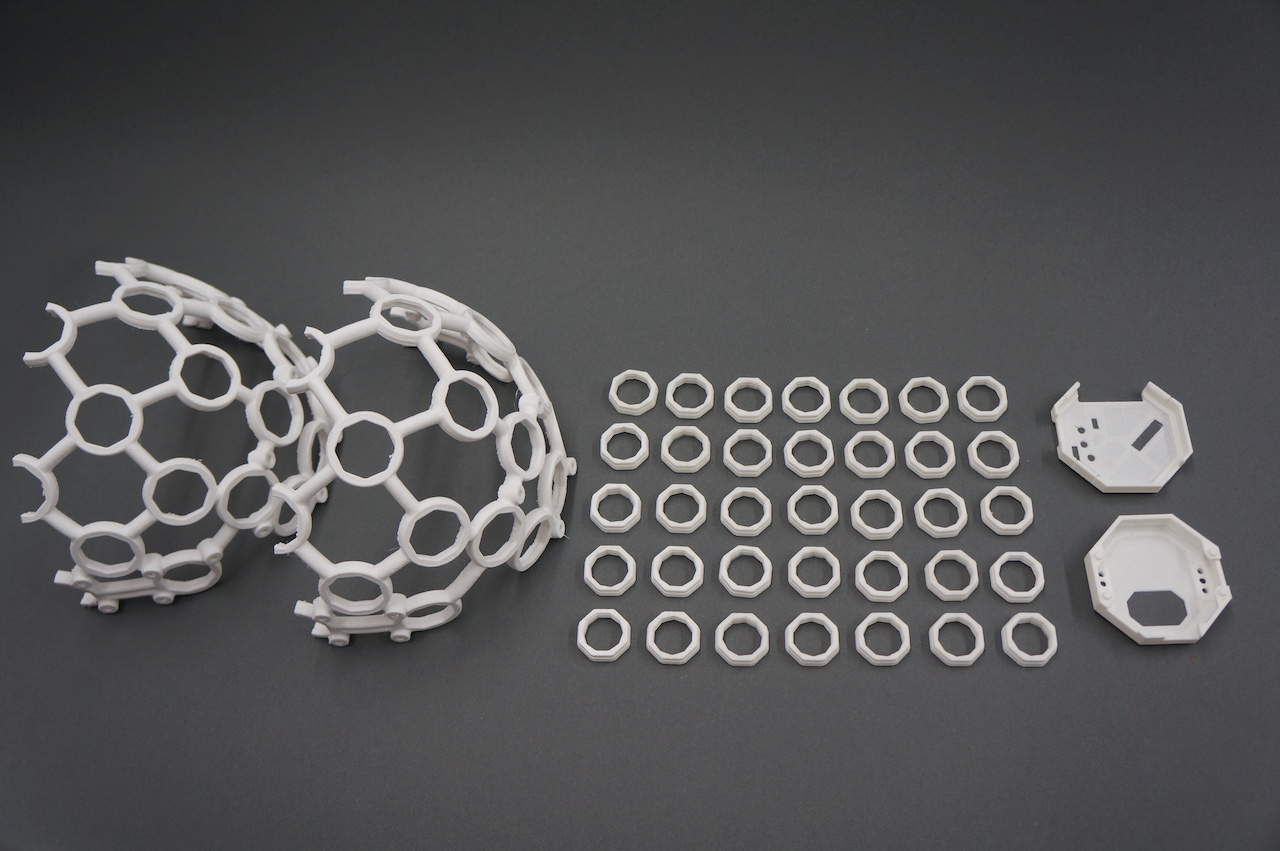
\includegraphics[width=1\textwidth]{Images/Imagenes/vinchamarkiv.png}\\
\end{center}

Además, al ser una compañía especializada en la creación de módulos de microcontroladores, nos proporcionaron orientación en cuanto a cómo realizar las conexiones entre la Raspberry Pi 4 que utilizamos y el sistema de filtrado EEG.

En los siguientes textos se adjuntan enlaces para ver la página oficial de OpenBCI y documentación de referencia correspondiente.

\begin{center}
    \href{https://openbci.com/}{Página oficial de OpenBCI}

    
    \href{https://docs.openbci.com/}{Documentación}

    
\end{center}

\begin{figure}[h!]
\centering

\begin{subfigure}[b]{0.45\linewidth}
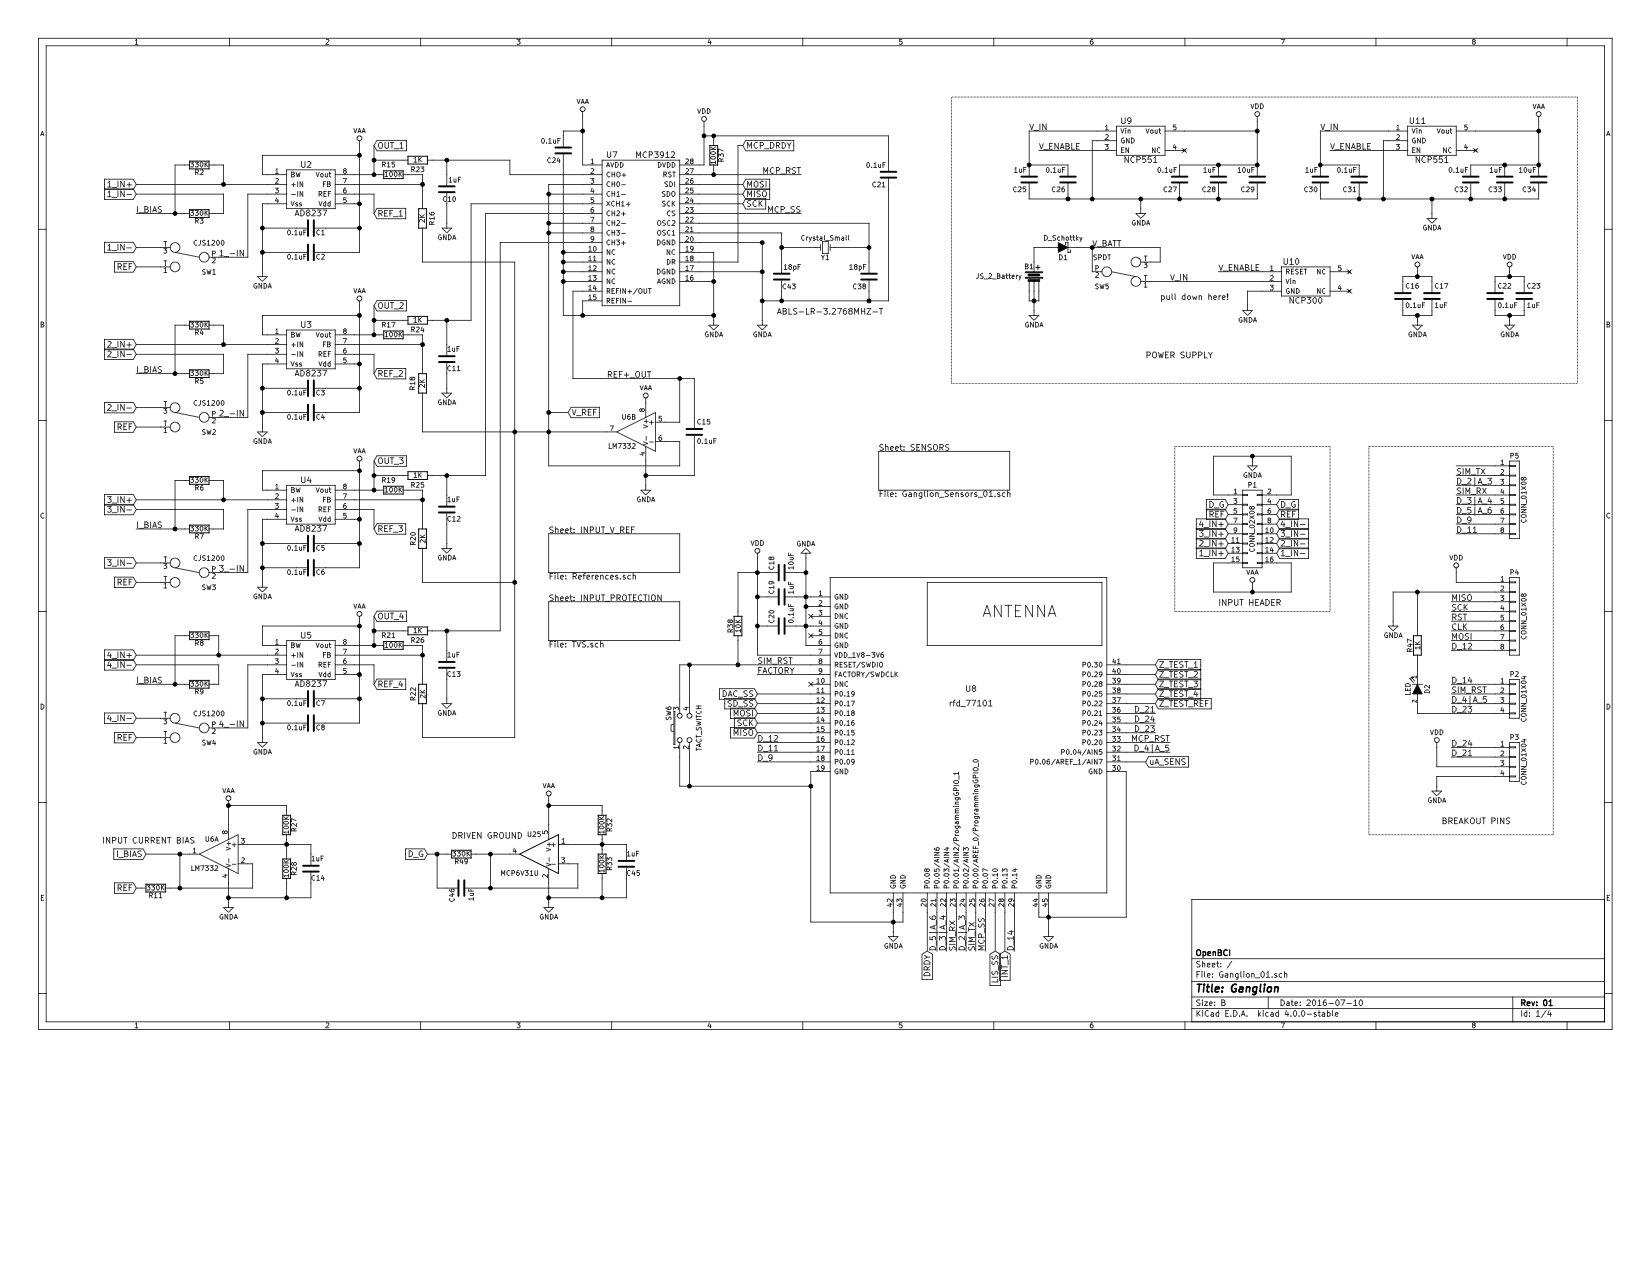
\includegraphics[width=\linewidth]{Images/Imagenes/esquematicodeganglion.png}
\caption{Diseño Esquemático}
\label{fig:westminster_lateral}
\end{subfigure}

\begin{subfigure}[b]{0.45\linewidth}
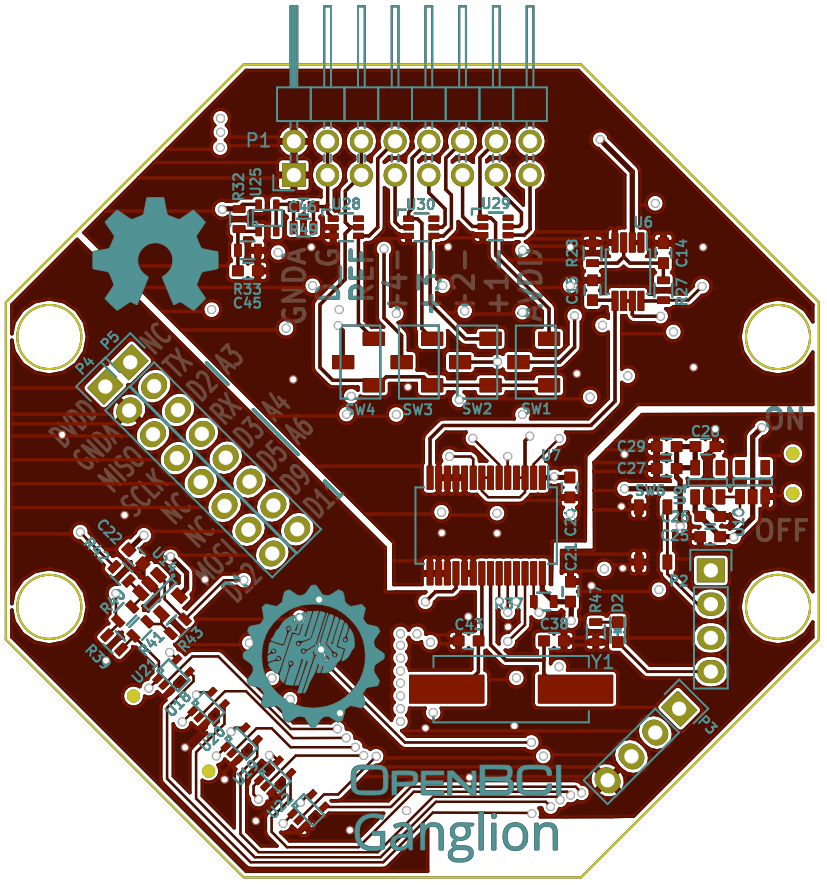
\includegraphics[width=\linewidth]{Images/Imagenes/pcbdeganglion.png}
\caption{Diseño PCB}
\label{fig:westminster_aerea}

\end{subfigure}
\caption{Diseño de microcontrolador de Open BCI}
\label{fig:westminster}
\end{figure}

\begin{center}
    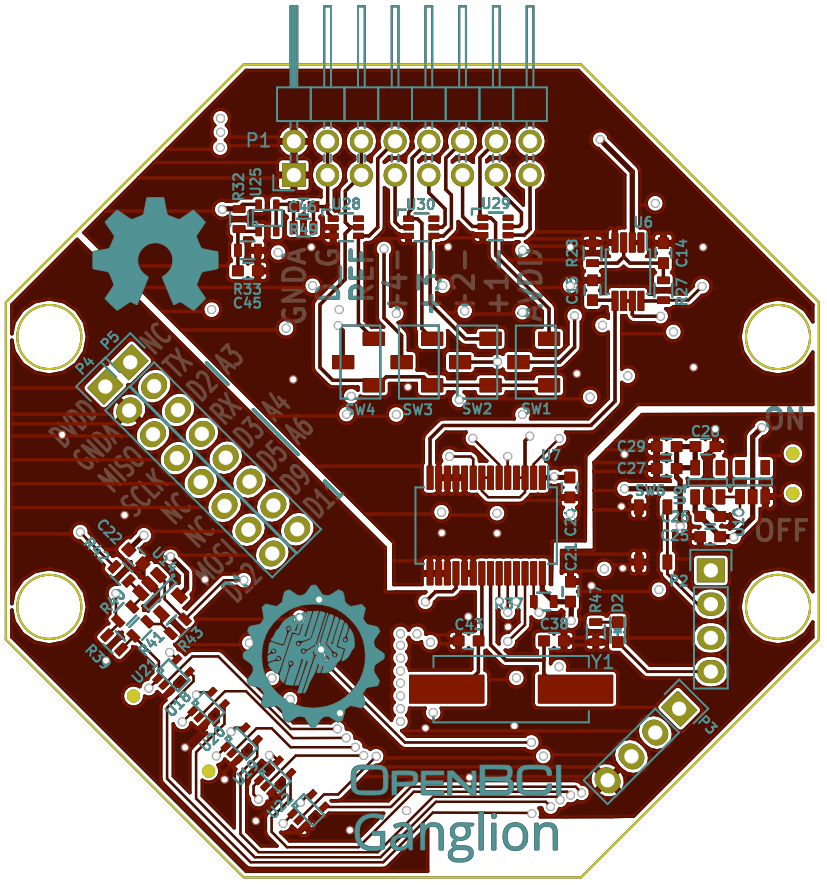
\includegraphics[width=1\textwidth]{Images/Imagenes/pcbdeganglion.png}\\

    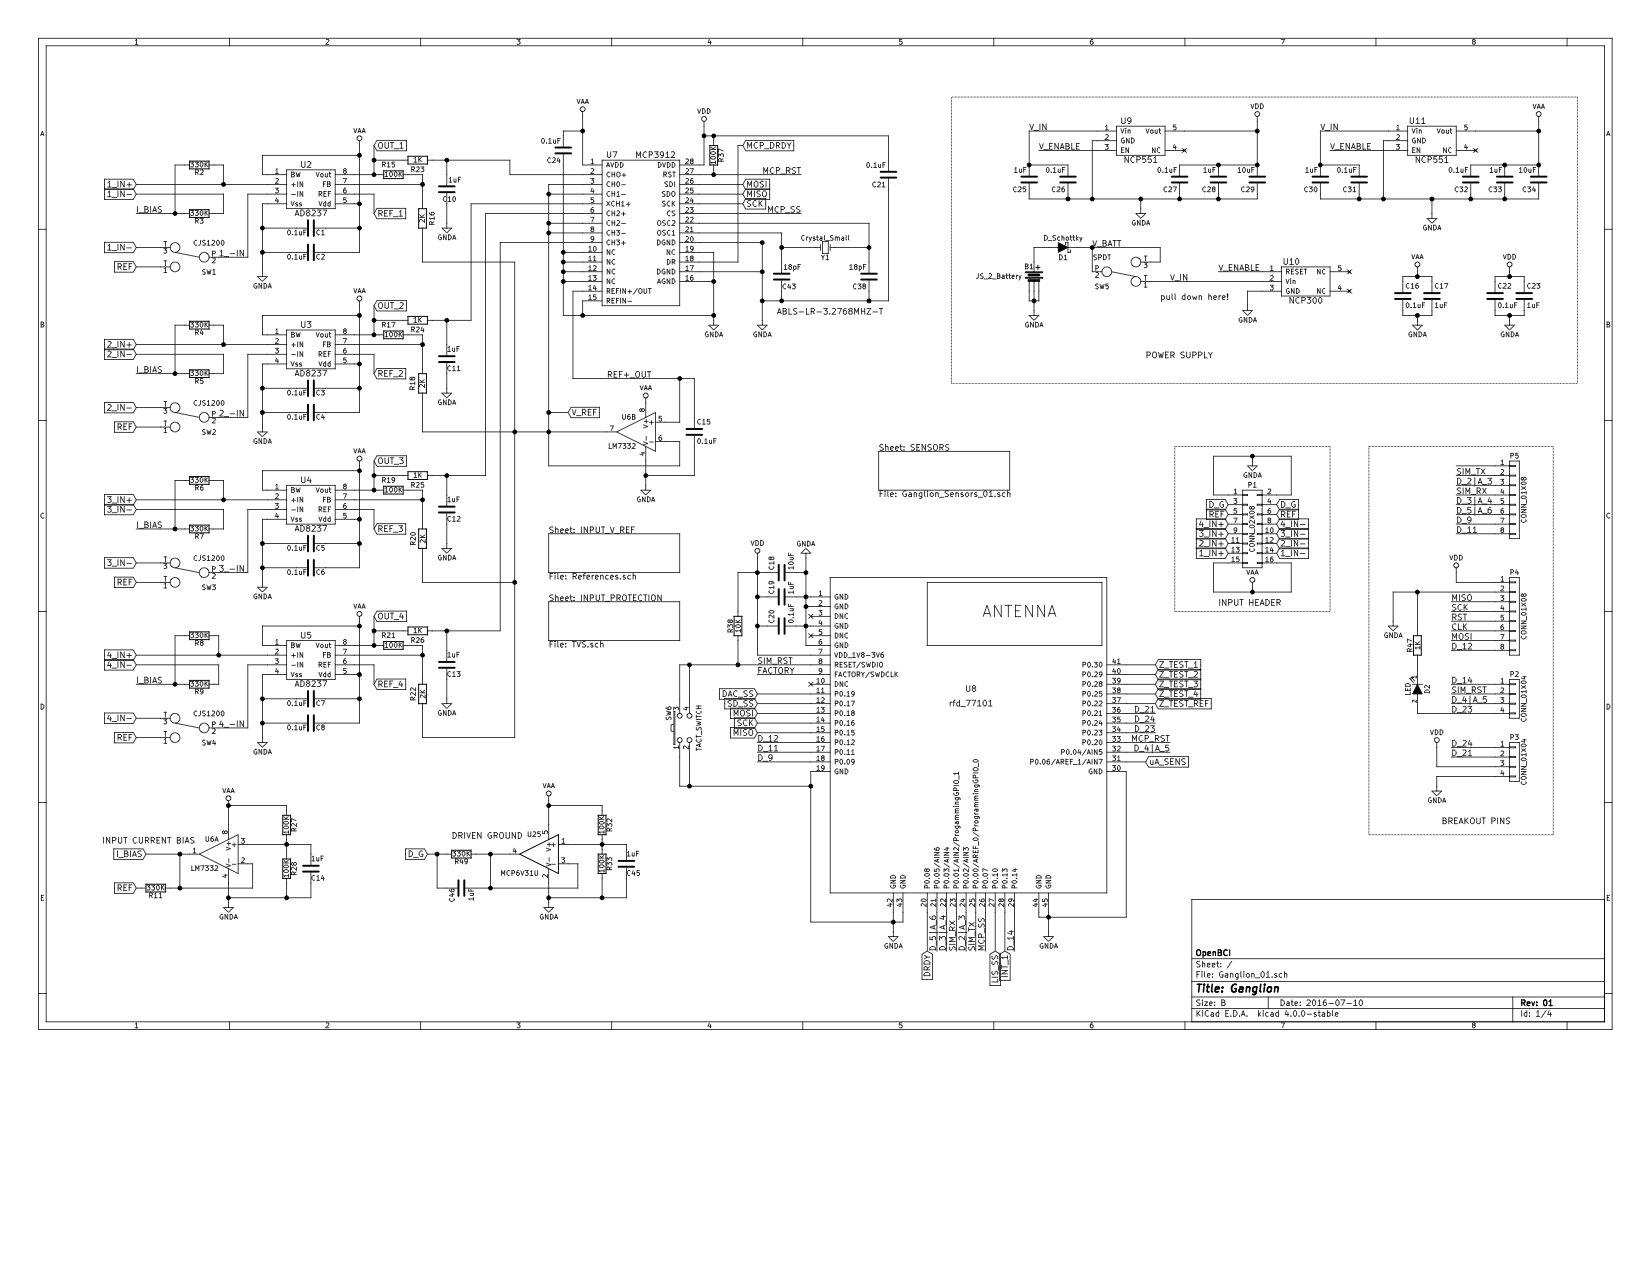
\includegraphics[width=1\textwidth]{Images/Imagenes/esquematicodeganglion.png}\\
\end {center}

\section{Desarrollo Teórico}
En este capítulo se describirán y desarrollarán todos los aspectos teóricos relacionados, justificando la elección de los componentes utilizados. Se abordarán teorías como la Jaula de Faraday y el sistema 10-20, además de ofrecer una explicación detallada sobre los tipos de señales empleadas, entre otros temas relevantes.

\subsection{Distinción de alimentaciones}

\subsection{¿Que es un electroencefalograma?}

Un electroencefalograma (EEG) es una prueba médica que registra la actividad eléctrica del cerebro. Esta actividad se mide a través de electrodos colocados en el cuero cabelludo, que detectan las señales eléctricas generadas por las neuronas mientras se comunican entre sí. Estas señales eléctricas se representan como ondas cerebrales en una gráfica que muestra diferentes frecuencias y patrones.

El EEG se utiliza comúnmente para:
\begin{itemize}
    \item \textbf{Diagnóstico de trastornos neurológicos:} Como la epilepsia, convulsiones, trastornos del sueño, encefalopatías o daño cerebral.
    \item \textbf{Monitoreo del estado cerebral:} En procedimientos quirúrgicos, cuidados intensivos o investigaciones sobre coma y muerte cerebral.
    \item \textbf{Investigación neurológica y cognitiva:} Para estudiar la actividad cerebral en respuesta a estímulos externos, emociones o en procesos de toma de decisiones.
    \item \textbf{Interfaz cerebro-computadora (BCI):} Donde se usa para traducir la actividad cerebral en comandos para controlar dispositivos externos, como en tu proyecto de silla de ruedas controlada por EEG.
    
\end{itemize}

Las ondas cerebrales se clasifican en varios tipos según su frecuencia: delta, theta, alpha, beta, y gamma, cada una asociada a diferentes estados de conciencia y actividades cerebrales.

Principalmente, a nosotros nos interesa el "Monitoreo del estado cerebral".

\subsection{¿Que es un EEG?}

Un electroencefalógrafo es un dispositivo médico que se utiliza para registrar y medir la actividad eléctrica del cerebro. Su función principal es captar las señales eléctricas generadas por las neuronas cerebrales y transformarlas en gráficos de ondas cerebrales, que se pueden analizar para evaluar la función cerebral.
\subsubsection{Componentes que tiene un EEG:}
\begin{itemize}
    \item \textbf{Electrodos:} Pequeños sensores que se colocan en el cuero cabelludo para captar los cambios de voltaje producidos por la actividad cerebral.
    \item \textbf{Amplificador:} Como las señales eléctricas del cerebro son muy débiles, el electroencefalógrafo incluye amplificadores que aumentan la señal para que sea lo suficientemente fuerte como para ser registrada.
    \item \textbf{Conversor analógico-digital:} Convierte las señales eléctricas captadas en un formato digital para su procesamiento por computadora.
    \item \textbf{Software de procesamiento:} El dispositivo utiliza un software que transforma las señales en gráficos de ondas cerebrales que se presentan en tiempo real en una pantalla o se registran para análisis posterior.
    \item \textbf{Pantalla/Gráficos:} El electroencefalógrafo muestra las señales eléctricas en forma de ondas, conocidas como ondas cerebrales (Delta, Theta, Alpha, Beta, Gamma), lo que permite a los médicos interpretar la actividad cerebral.
\end{itemize}

\subsection{Sistema 10-20}

El sistema 10-20 es un método internacionalmente estandarizado para la colocación de electrodos en el cuero cabelludo durante un electroencefalograma (EEG). Este sistema asegura que los electrodos se coloquen de manera uniforme y precisa en relación con los puntos anatómicos del cráneo, permitiendo una medición consistente y reproducible de la actividad eléctrica cerebral.

El nombre "10-20" proviene de las distancias porcentuales entre los electrodos: Los electrodos se colocan en posiciones que están al 10\% o al 20\% de la distancia total entre puntos anatómicos clave del cráneo.
Puntos anatómicos clave de referencia:
\begin{itemize}
    \item \textbf{Nasion:} El punto entre la frente y la nariz.
    \item \textbf{Inion:} El punto más prominente en la parte posterior de la cabeza.
    \item \textbf{Puntos preauriculares:} Justo por encima de los oídos, a cada lado de la cabeza.
\end{itemize}

Las posiciones de los electrodos se distribuyen sobre la cabeza tomando como referencia estos puntos para cubrir todo el cuero cabelludo de forma equidistante.

\subsubsection{¿Para qué sirve?}
El sistema 10-20 se utiliza para garantizar una colocación precisa y consistente de los electrodos en los estudios de EEG. Algunos de sus beneficios incluyen:

\begin{itemize}

    \item \textbf{Estandarización global:} Permite que los estudios de EEG sean comparables en diferentes laboratorios y entre diferentes pacientes.
    \item \textbf{Cobertura completa del cerebro:} El sistema asegura que se cubran adecuadamente diferentes áreas del cerebro (frontal, parietal, occipital, temporal).
    \item \textbf{Detección de anomalías:} Facilita la identificación de regiones del cerebro donde pueden estar ocurriendo fenómenos anormales, como descargas epilépticas, actividad lenta anormal o asimetrías en las ondas cerebrales.
    
\end{itemize}

\subsubsection{¿Como se aplica?}

En un estudio de EEG, se colocan electrodos en el cuero cabelludo siguiendo estas posiciones predeterminadas en el sistema 10-20:

\begin{enumerate}
    \item Puntos y nomenclatura: Cada posición de electrodo tiene una nomenclatura que se utiliza para identificar las regiones del cerebro de las que se está registrando la actividad.
\end{enumerate}

\begin{itemize}
    \item F: Frontal (F3, F4, Fz, etc.)
    \item C: Central (C3, C4, Cz, etc.)
    \item P: Parietal (P3, P4, Pz, etc.)
    \item O: Occipital (O1, O2)
    \item T: Temporal (T3, T4, etc.)
    \item Los números impares (1, 3, 5, 7) se asignan al hemisferio izquierdo, mientras que los números pares (2, 4, 6, 8) se asignan al hemisferio derecho. La letra "z" indica posiciones centrales (a lo largo de la línea media de la cabeza).
\end{itemize}

\subsubsection{Pasos para aplicar el sistema 10-20}

\begin{enumerate}

    \item \textbf{Medición del cráneo:} Se mide la distancia desde el nasion al inion y desde un punto preauricular al otro. Luego, se calculan los puntos intermedios en un 10 o 20 de esas distancias para determinar las ubicaciones exactas de los electrodos.
    
    \item \textbf{Colocación de los electrodos:} Se colocan electrodos en los puntos marcados, asegurando una cobertura uniforme de la cabeza. Esto puede hacerse usando una gorra de EEG con posiciones ya marcadas o mediante la medición manual.
    
    \item \textbf{Registro de la actividad:} Una vez colocados los electrodos, se inicia el registro de la actividad cerebral. Los electrodos miden las diferencias de potencial eléctrico entre las regiones del cerebro cubiertas por los electrodos.
\end{enumerate}

\subsubsection{Aplicaciones del sistema 10-20}
\begin{itemize}
    \item \textbf{Diagnóstico clínico:} El sistema se usa comúnmente en estudios de EEG para diagnosticar condiciones neurológicas como la epilepsia, trastornos del sueño, y daño cerebral.
    \item \textbf{Investigación:} En estudios de neurociencia, el sistema 10-20 facilita la comparación de la actividad cerebral entre sujetos, ya que la ubicación de los electrodos está estandarizada.
    \item \textbf{Interfaces cerebro-computadora (BCI):} En proyectos de BCI, se utiliza el sistema 10-20 para colocar electrodos en áreas específicas del cerebro que controlan movimientos o funciones específicas.
\end{itemize}


\subsection{Comunicación UART}

El UART (Universal Asynchronous Receiver-Transmitter) es un periférico de hardware utilizado para la comunicación serie. Su principal función es permitir la transmisión y recepción de datos de manera asíncrona, lo que implica que no requiere de una señal de clock compartida entre el transmisor y el receptor. A continuación, se destacan las características principales de este tipo de comunicación:

\begin{itemize}
    \item \textbf{Comunicación serie:} Los datos se transmiten de forma secuencial, bit a bit, a través de una línea de transmisión (TX) y se reciben mediante una línea de recepción (RX).
    \item \textbf{Asincronía:} Al no utilizar una señal de clock constante, ambos dispositivos deben estar configurados con la misma velocidad de transmisión (tasa de baudios) para asegurar la correcta recepción de los datos.
    \item \textbf{Formato de datos:} Cada paquete de datos transmitido generalmente incluye un bit de inicio (indicando el comienzo de la transmisión), entre 5 y 9 bits de datos, un bit opcional de paridad (para detección de errores), y uno o dos bits de parada.
    \item \textbf{Velocidad de transmisión:} La velocidad de transmisión de la información, conocida como tasa de baudios, se refiere al número de bits transmitidos por segundo.
\end{itemize}

La implementación de la comunicación UART en nuestro proyecto se utiliza para la recepción y procesamiento de señales. Específicamente, en la RP2040 Zero, enviamos las lecturas de los cuatro canales del ADC (Conversor Analógico-Digital) en formato JSON durante un período de tiempo definido y con una frecuencia de muestreo específica a la Raspberry Pi 4.

\subsection{Gráfico de Fourier}
El gráfico de Fourier está basado en la Transformada de Fourier (TF), que es una operación matemática que descompone una señal en sus componentes sinusoidales de diferentes frecuencias. Este método es especialmente útil para analizar señales periódicas y no periódicas.

La Transformada de Fourier dicta que: 

Dada una señal \textit{x(t)} en el dominio del tiempo, la transformada de Fourier \textit{X(f)} se define como:

\begin{figure}[H]
    \centering
    \includegraphics[width=0.5\linewidth]{Images//Formulas/FormulaFourier.png}
    \caption{Formula de Transformada de Fourier}
    \label{fig:enter-label}
\end{figure}

Donde:
\begin{itemize}
    \item \textit{x(t)} es la señal en el dominio del tiempo.
    \item \textit{X(f)} es la señal transformada en el dominio de la frecuencia.
    \item \textit{f} es la frecuencia (Hz).
    \item \textit{j} es la unidad imaginaria 
    \item $e^{-j2\pi ft}$ es la función compleja que representa la descomposición en sinusoides.

\end{itemize}

El gráfico de Fourier representa la magnitud o la fase de la transformada de Fourier. Este gráfico tiene dos componentes importantes:

\begin{enumerate}
    \item \textbf{Espectro de Magnitud:} Se representa gráficamente la magnitud de cada frecuencia presente en la señal. En el eje horizontal está la frecuencia \textit{f}, y en el eje vertical está la magnitud |\textit{X(f)}|, que indica cuánta energía o potencia de la señal está concentrada en esa frecuencia específica.

    \begin{equation}
        |X(f)| = \sqrt{Re(X(f))^2+Im(X(f))^2}
    \end{equation}
    
    \item \textbf{Espectro de Fase:} Indica el desfase de cada frecuencia con respecto a la señal original. En el eje horizontal también está la frecuencia \textit{f}, y en el eje vertical está el ángulo de fase \textit{\theta(f)}, que puede calcularse como:

    \begin{equation}
        \theta = tan^{-1} \left(\frac{Im(X(f))}{a}\right)
        \label{eq:1}
    \end{equation}
\end{enumerate}

\subsubsection{¿Para que sirve?}
El grafico de Fourier es una herramienta que sirve para analizar señales en el dominio de la frecuencia.
\begin{enumerate}
    \item \textbf{Análisis de frecuencias:}
    \begin{itemize}
        \item \textbf{Descomposición de señales complejas:} Permite descomponer una señal en sus componentes de frecuencia individuales. Esto es útil cuando quieres saber qué frecuencias están presentes en una señal y su importancia relativa.
    
        \item \textbf{Identificación de frecuencias dominantes:} El gráfico te muestra cuáles son las frecuencias que más contribuyen a la señal original, lo que es esencial para entender fenómenos periódicos y patrones.
    \end{itemize}
    \item \textbf{Filtrado de señales:}
    \begin{itemize}
        \item \textbf{Diseño de filtros:} Si necesitas eliminar ruido o componentes no deseados de una señal, el gráfico de Fourier ayuda a identificar las frecuencias del ruido o interferencia. Luego puedes diseñar un filtro que elimine esas frecuencias.
    
        \item \textbf{Filtrado de bandas:} Puedes aplicar filtros pasa-bajas, pasa-altas o de banda (pasa-banda o elimina-banda) a una señal. El gráfico te muestra exactamente qué frecuencias están siendo afectadas.
    \end{itemize}
    
    \item \textbf{Compresión de datos:}
    \begin{itemize}
        \item \textbf{ Eliminación de información redundante:} En algunas señales (como imágenes o audio), las frecuencias más altas o muy bajas pueden no ser necesarias. Usando el gráfico de Fourier, puedes identificar esas frecuencias y eliminarlas para comprimir los datos sin perder información relevante.
    
        \item \textbf{Compresión de audio e imágenes:} Muchos algoritmos de compresión (como JPEG o MP3) utilizan la Transformada de Fourier o versiones discretas de ella para eliminar componentes de alta frecuencia que son menos perceptibles para el ser humano.
    \end{itemize}
    
    \item \textbf{Análisis de vibraciones y ondas:}
    \begin{itemize}
        \item \textbf{Detección de fallos en maquinaria:} En ingeniería mecánica y de control, el gráfico de Fourier es utilizado para analizar vibraciones y detectar problemas como desbalances, resonancias, o desgastes en partes móviles. Las frecuencias anómalas pueden señalar fallos.
    
        \item \textbf{Análisis de señales acústicas:} Permite estudiar el espectro de frecuencias en señales de audio. Por ejemplo, para identificar las características de sonidos musicales o voces.
    \end {itemize}
    
    \item \textbf{Procesamiento de señales EEG:}
    \begin{itemize}
        \item Para el análisis de señales cerebrales (EEG), el gráfico de Fourier es vital para identificar y separar las diferentes bandas de frecuencias asociadas con diferentes actividades cerebrales (como las ondas delta, theta, alpha, beta y gamma).
    
        \item \textbf{Monitoreo de actividad cerebral:} En neurociencia, el análisis de Fourier se utiliza para analizar patrones de actividad cerebral, detectar anormalidades y realizar interfaces cerebro-máquina (como el control de la silla de ruedas en tu proyecto).
    \end{itemize}
    \item \textbf{Análisis de señales en telecomunicaciones:}
    \begin{itemize}
        \item \textbf{Ancho de banda:} El gráfico de Fourier permite determinar el ancho de banda necesario para transmitir una señal sin pérdida de información.
    
        \item \textbf{Modulación y demodulación:} En sistemas de comunicaciones, la modulación de señales se realiza en el dominio de la frecuencia. El gráfico de Fourier te permite visualizar cómo una señal ha sido modulada para su transmisión y cómo se puede demodular para su interpretación.
    \end{itemize}
    \item \textbf{Análisis de imágenes:}
    \begin{itemize}
        \item \textbf{Reconocimiento de patrones:} En procesamiento de imágenes, la transformada de Fourier se utiliza para identificar patrones repetitivos o estructuras de frecuencia en una imagen. Es útil en tareas como la detección de bordes o compresión de imágenes.
    
        \item \textbf{Eliminación de ruido:} Permite eliminar patrones específicos de ruido en imágenes filtrando frecuencias indeseadas.
    \end{itemize}
\end{enumerate}

\subsection{Filtros digitales}

Un filtro digital es una herramienta utilizada en el procesamiento de señales para modificar o mejorar ciertos aspectos de una señal digital, eliminando o atenuando componentes no deseados, como ruido, o destacando componentes útiles. Los filtros digitales operan sobre señales discretizadas (muestreadas) y utilizan algoritmos matemáticos para realizar diversas transformaciones.

Existen diferentes tipos de filtros digitales, según su función:

\begin{itemize}
    \item \textbf{Filtro pasa bajas:} Permite el paso de frecuencias bajas y atenúa las frecuencias altas.
    \item \textbf{Filtro pasa altas:} Permite el paso de frecuencias altas y atenúa las bajas.
    \item \textbf{Filtro pasa banda:} Permite el paso de un rango específico de frecuencias.
    \item \textbf{Filtro elimina banda (Notch):} Atenúa un rango específico de frecuencias, como en el caso de eliminar interferencias a 50-60 Hz.
\end{itemize}

Los filtros digitales pueden ser FIR (Finite Impulse Response) o IIR (Infinite Impulse Response):

\begin{itemize}
    \item Los filtros FIR tienen una respuesta finita y son más estables, pero pueden necesitar más recursos de procesamiento.
    \item Los filtros IIR tienen una respuesta infinita y suelen ser más eficientes en términos de recursos, pero pueden ser menos estables si no se diseñan correctamente.
\end{itemize}

Los filtros digitales son ampliamente usados en aplicaciones como procesamiento de audio, señales biológicas (como EEG), imágenes y telecomunicaciones.
\subsubsection{¿Para que los necesitamos si ya tenemos por Hardware?}
La combinación de filtros físicos (implementados en hardware) con filtros digitales (implementados en software) presenta una serie de ventajas significativas, incluso si ya se han instalado filtros físicos en el sistema. Aunque los filtros basados en hardware permiten un filtrado efectivo de las señales EEG, los filtros digitales proporcionan una flexibilidad y capacidades adicionales que no siempre son posibles de lograr mediante hardware exclusivamente. A continuación, se detallan las razones por las cuales puede ser beneficioso incorporar filtros digitales a la salida de los filtros físicos:
\begin{enumerate}
    \item \textbf{Ajuste Preciso y Mayor Flexibilidad}
    
    Los filtros de hardware están limitados a sus parámetros iniciales, ya que una vez construidos con componentes específicos (como resistencias, condensadores, etc.), sus características clave, tales como la frecuencia de corte y el ancho de banda, son difíciles de modificar. En contraste, los filtros digitales permiten ajustar fácilmente parámetros como la frecuencia de corte o la configuración de filtrado sin necesidad de realizar cambios físicos. Esto resulta especialmente útil cuando, tras el análisis de la señal, es necesario ajustar el rango de paso de un filtro o eliminar una frecuencia no contemplada inicialmente. Además, los filtros digitales permiten realizar modificaciones rápidas y sin intervención física, optimizando la eficiencia del proceso.
    \item \textbf{Compensación de las Limitaciones Intrínsecas del Hardware}
    
    Los filtros físicos, aunque efectivos, no son perfectos. Su desempeño puede verse afectado por tolerancias en los componentes o por factores ambientales, como la temperatura y el envejecimiento de los mismos. Los filtros digitales, por su parte, pueden corregir o complementar las imperfecciones de los filtros de hardware. Por ejemplo, si un filtro físico no consigue eliminar completamente el ruido de 50 Hz o presenta desviaciones mínimas en las frecuencias de corte, un filtro digital puede ajustarse con precisión para corregir estas deficiencias, mejorando así la calidad general del filtrado.
    \item \textbf{Filtrado Adaptativo en Tiempo Real}
    
    Los filtros físicos son estáticos, lo que significa que su comportamiento es constante y no varía según las condiciones de la señal. En cambio, un filtro digital ofrece la posibilidad de implementar técnicas de filtrado adaptativo, es decir, que el filtro ajuste sus características en función de las condiciones cambiantes de la señal. Esto es especialmente beneficioso en entornos donde las condiciones son variables, como cuando la interferencia de 50 Hz no está presente de manera constante. Un filtro digital adaptativo puede activarse solo cuando detecta interferencias, optimizando el procesamiento de la señal en tiempo real. De esta manera, el sistema EEG se ajusta de manera dinámica, lo que puede incrementar la fiabilidad del procesamiento.
    \item \textbf{Procesamiento Avanzado y Filtrado de Alta Precisión}
    
    La complejidad de los filtros físicos está limitada por los componentes que los conforman. Sin embargo, en el ámbito digital es posible implementar filtros de mayor complejidad y orden, permitiendo un filtrado más preciso y específico. Los filtros digitales de mayor orden ofrecen transiciones más nítidas entre las bandas de paso y de rechazo. Por ejemplo, con un filtro digital, es posible eliminar una banda estrecha de ruido sin afectar las frecuencias adyacentes de interés, algo difícil de lograr mediante componentes físicos convencionales.
    \item \textbf{Filtrado en Múltiples Etapas}
    
    El uso de filtrado digital permite procesar la señal en diferentes etapas, lo que resulta en un análisis más profundo y detallado de las señales EEG. Tras el paso por los filtros físicos, se pueden aplicar diferentes tipos de filtros digitales para aislar aspectos específicos de la señal que no fueron manejados por el filtrado físico. Por ejemplo, se pueden implementar filtros pasa banda específicos para resaltar ciertas bandas de ondas cerebrales, como las ondas alpha o beta, o utilizar técnicas avanzadas como el Análisis de Componentes Independientes (ICA) para separar señales superpuestas o interferencias no deseadas. El uso de filtros adaptativos también permite ajustar continuamente la respuesta del sistema, optimizando el rendimiento del procesamiento de señales.
    \item \textbf{Posprocesamiento y Análisis Selectivo}
    
    El filtrado digital permite realizar un análisis detallado de las señales EEG en una etapa posterior, ya sea sobre los datos almacenados o sobre la señal adquirida en tiempo real. Este posprocesamiento es fundamental para detectar patrones específicos o eliminar artefactos que no fueron suficientemente atenuados en la etapa inicial de filtrado físico. Por ejemplo, los artefactos relacionados con el movimiento o las señales de baja frecuencia, como la respiración, pueden requerir un ajuste adicional después de la adquisición de la señal. Además, un análisis más exhaustivo en tiempo real puede detectar elementos que los filtros de hardware no lograron capturar completamente.
    \item \textbf{Redundancia y Seguridad}
    
    Incorporar tanto filtros físicos como digitales en un sistema de procesamiento de señales EEG añade una capa extra de seguridad. Si un filtro físico falla o no cumple completamente su función, el filtro digital actúa como un sistema de respaldo, asegurando que el ruido y las interferencias no afecten el análisis de la señal. Esta redundancia es clave en entornos críticos donde se necesita garantizar la integridad y pureza de los datos EEG para obtener resultados confiables y precisos.
\end{enumerate}


\subsection{Cantidad de canales}

\subsection{Gel conductor}
El gel conductor neutro empleado en los electroencefalogramas (EEG) es una sustancia formulada para optimizar la conductividad eléctrica entre los electrodos y el cuero cabelludo del paciente. Su principal objetivo es minimizar la resistencia entre los electrodos y la piel, garantizando una transmisión eficiente y sin interferencias de las señales eléctricas cerebrales hacia los electrodos. 

\subsubsection{Cómo aplicar el gel conductor}
En los electrodos de copa dorada, el procedimiento consiste únicamente en rellenar la cavidad de la copa con el gel conductor, posteriormente colocarlo sobre una zona del cuero cabelludo previamente limpiada con algodón, mantenerlo en posición durante unos segundos y eliminar cualquier exceso de gel, en caso de haberlo, con un pequeño trozo de papel. Utilizamos este gel en el proyecto con el fin de obtener la mejor calidad posible en las señales, además de generar un leve efecto de succión que contribuye a mantener los electrodos firmemente adheridos.

\subsection{Jaula de Faraday}
Una jaula de Faraday es, esencialmente, una estructura metálica diseñada para proteger su interior de los campos eléctricos estáticos. Su nombre proviene del físico Michael Faraday, quien construyó la primera de estas estructuras en 1836. Las jaulas de Faraday se utilizan para proteger su contenido de descargas eléctricas y del ruido electromagnético, debido a que, en su interior, el campo eléctrico es nulo. Su principio de funcionamiento se basa en las propiedades de un conductor en equilibrio electrostático, lo que impide que cualquier carga eléctrica atraviese la estructura. Por esta razón, se emplean para proteger dispositivos sensibles a las cargas eléctricas. Este fenómeno es conocido como apantallamiento eléctrico.

\subsubsection{¿Por qué utilizamos una Jaula de Faraday?}
Dado que trabajamos con señales altamente susceptibles al ruido debido a su frecuencia y voltaje, como es el caso de las señales captadas por el EEG, es fundamental mantenerlas lo más aisladas posible de interferencias externas. Además, contamos con una fuente importante de ruido electromagnético: el motor. Por esta razón, es esencial posicionar los componentes lo más alejados posible entre sí y utilizar una Jaula de Faraday en la sección destinada a la recepción y procesamiento de las señales.

La implementación de este elemento se realiza mediante una caja metálica que será ubicada en la parte superior trasera de la silla de ruedas, es decir, en la zona de apoyo de la espalda, para mantenerla lo más distante posible de los motores.

\subsection{Utilización de Offsets}
En la sección de procesamiento y recepción, utilizamos 

\subsection{Sistema de emergencia}

\subsection{Tipos de alimentaciones}

\subsection{Sistema de control}

\subsection{Puentes H}
Un Puente H es un circuito utilizado para invertir el sentido de giro de un motor y para separar su etapa de potencia con la de control. Su nombre viene de la forma gráfica que tiene el circuito. Se construye con 4 interruptores, pueden ser mecánicos o transistores. En la siguiente imágen se puede ver la forma de un puente H.

\begin{figure}[H]
    \centering
    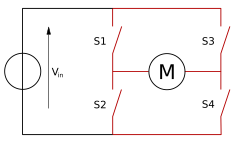
\includegraphics[width=0.5\linewidth]{Images/PuenteH/H_bridge.svg.png}
    \caption{Puente H Genérico por medio de llaves mecánicas}
\end{figure}

En este ejemplo, cuando la llave S1 y S4 se cierran, correrá corriente por esta rama, haciendo que el motor funcione y tenga un sentido de giro. Cuando la llave S2 y S3 se cierran, correrá corriente por esta rama también, pero con sentido de giro invertido. En este circuito, S1 y S2 nunca pueden estar cerradas al mismo tiempo, porque esto generaría un corto circuito, lo mismo con las llaves S3 y S4.

\begin{figure}[H]
    \centering
    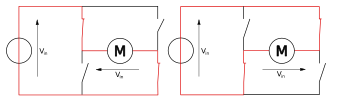
\includegraphics[width=0.70\linewidth]{Images/PuenteH/H_bridge_operating.svg.png}
    \caption{Puente H Operando}
\end{figure}

\subsubsection{Puente H de potencia}
Un puente H de potencia es un tipo de circuito en el que la etapa de potencia, que incluye el motor, los transistores y está conectada a altas tensiones y corrientes, se encuentra separada de la etapa de control, la cual generalmente opera con voltajes más bajos. Esta separación se realiza para proteger la etapa de control de las altas tensiones, que podrían dañar o quemar sus circuitos. Podemos utilizar nuestro puente H como ejemplo para ilustrar este concepto:

 \begin{figure}[H]
     \centering
     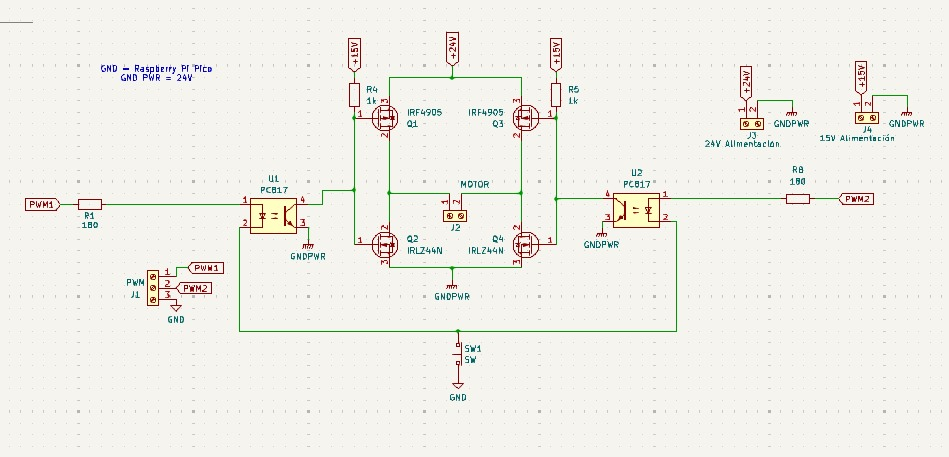
\includegraphics[width=0.85\linewidth]{Images/PuenteH/WhatsApp Image 2024-08-28 at 9.05.56 AM.jpeg}
     \caption{Nuestro Puente H de potencia}
     \label{fig:enter-label}
 \end{figure}

En nuestro puente H, hemos separado las ramas del motor de las de control, ya que el motor opera con 24V DC y tiene una corriente eficaz de 3,5A. Para controlar el motor de manera eficiente, hemos optado por un diseño que incluye cuatro transistores MOSFET de potencia, los cuales pueden soportar picos de hasta 74A y 82A, garantizando que puedan manejar la corriente del motor de manera continua. Además, los transistores son controlados mediante señales PWM, las cuales atraviesan un optoacoplador para minimizar el riesgo de que la corriente del motor regrese a la placa de control y cause daños. De ésta manera, podemos controlar el giro del motor de manera segura y regulada.


\subsection{Sistema de recepción de señales}

\subsection{Control por PWM}
La modulación por ancho de pulso (PWM, por sus siglas en inglés Pulse Width Modulation) es una técnica empleada para regular la cantidad de energía suministrada a una carga, como un motor o un LED, mediante la variación del ciclo de trabajo de una señal pulsante. En lugar de modificar el voltaje de forma continua, PWM ajusta el tiempo durante el cual la señal permanece en estado alto (encendida) y bajo (apagada) dentro de un período fijo. Esto depende de los siguientes parámetros:

\begin{itemize}
    \item \textbf{Frecuencia:} Se refiere a la cantidad de ciclos de encendido y apagado que ocurren en un segundo, y se mide en Hertz (Hz).
    \item \textbf{Ciclo de trabajo:} Es el porcentaje de tiempo que la señal se mantiene en estado alto durante un ciclo. Por ejemplo:
    Un ciclo de trabajo del 0\% implica que la señal está siempre apagada.
    Un ciclo de trabajo del 50\% significa que la señal está encendida la mitad del tiempo y apagada la otra mitad.
    Un ciclo de trabajo del 100\% indica que la señal permanece siempre encendida.
    En nuestro proyecto, aplicamos la técnica de PWM en el control de los motores. Dado que utilizamos dos motores, si estos operaran a su máxima potencia, la silla de ruedas se desplazaría a una velocidad excesiva. Por esta razón, empleamos un ciclo de trabajo del 25\% para limitar la velocidad de avance.
\end{itemize}

\section{Desarrollo Técnico}
En este capítulo se proporcionará una descripción detallada sobre el funcionamiento de los distintos circuitos que conforman el dispositivo, así como su interacción en conjunto para cumplir con los objetivos del proyecto. Se explicará de manera clara y concisa cómo se utiliza el dispositivo, incluyendo instrucciones específicas para su correcto manejo y operatividad.

Además, se incluirán datos técnicos relevantes, tales como especificaciones de los componentes, características del diseño, y cualquier otro detalle que sea esencial para la comprensión del sistema. También se abordarán aspectos importantes acerca de las partes constitutivas del dispositivo, su función dentro del esquema general, y las consideraciones necesarias para su mantenimiento y optimización.

\subsection{Descripción del funcionamiento}
El usuario se sienta en la silla de ruedas y se coloca el dispositivo EEG. El EEG capta las señales cerebrales (alfa, beta, gamma, delta y theta) y las somete a un proceso de filtrado por hardware que incluye un filtro notch de 50 Hz, un filtro pasa-bajo de 100 Hz, un filtro pasa-alto de 0,5 Hz y un segundo filtro notch de 50 Hz. Posteriormente, las señales pasan por un circuito de compensación de offset para poder realizar la lectura por parte de la RP2040 Zero ya que la misma no puede leer valores negativos. Esta unidad se encarga de leer los datos mediante cuatro canales de ADC y enviarlos a la Raspberry Pi 4 por protocolo UART, donde se aloja el programa principal para el funcionamiento de la silla de ruedas.

Entre estos códigos se encuentran el control de motores, los filtros digitales, el procesamiento de señales y la inteligencia artificial (IA). Una vez las señales llegan a la Raspberry Pi 4, se filtran digitalmente para eliminar el ruido y mejorar la calidad de los datos. Tras el filtrado, las señales se envían a la IA, que tiene la función de reconocer los patrones cerebrales y determinar la dirección en la que el usuario desea moverse. Una vez el patrón ha sido identificado, se envía una señal a los motores para dirigir la silla hacia la dirección deseada (adelante, atrás, izquierda o derecha).

Además, el proyecto incluye un sistema de emergencia diseñado para garantizar la seguridad del usuario. Este sistema se activa si se detecta un error en la lectura de las señales o si hay un obstáculo en la trayectoria deseada. Su objetivo es prevenir accidentes y aumentar la seguridad del usuario al utilizar la silla de ruedas.

El sistema de emergencia utiliza sensores de ultrasonido para detectar la presencia de objetos a menos de 20 cm de la silla. En caso de detección, el sistema frena los motores y activa un LED en la dirección del objeto, además de un buzzer que emite una señal sonora durante un breve período para alertar al usuario sobre la activación del sistema.

\subsection{Funcionamiento del EEG}

El sistema de control de nuestra silla de ruedas se basa en el reconocimiento de señales cerebrales, lo que requiere un dispositivo especializado para captarlas: el electroencefalograma (EEG). Hemos desarrollado un EEG en forma de una cofia equipada con electrodos, los cuales se colocan siguiendo el protocolo conocido como “Sistema 10-20”. Este sistema estándar de ubicación define puntos específicos en el cuero cabelludo donde se deben colocar los electrodos para obtener lecturas óptimas de la actividad cerebral.

Los electrodos actúan como sensores pasivos que detectan las ondas cerebrales producidas por la actividad eléctrica del cerebro. Estas ondas se manifiestan como pequeñas fluctuaciones en el voltaje, que son captadas por los electrodos cuando se colocan sobre la superficie del cuero cabelludo del usuario. Es importante destacar que estos electrodos no penetran en el cráneo ni interactúan directamente con las neuronas. En cambio, registran los potenciales eléctricos generados por la actividad cerebral subyacente que se propagan hasta la superficie del cuero cabelludo.

Debido a que las señales captadas por los electrodos son de muy baja amplitud, requieren ser amplificadas antes de su procesamiento. Este paso no solo amplifica la señal cerebral, sino también el ruido presente en el entorno o generado por el propio cuerpo. Para abordar este problema, se realiza un proceso de filtrado que elimina el ruido y permite aislar las frecuencias relevantes de las ondas cerebrales.

Las frecuencias de las ondas cerebrales detectadas son las siguientes:

\begin{itemize}
    \item Ondas alfa: 8-12 Hz
    \item Ondas beta: 12-30 Hz
    \item Ondas gamma: 30-100 Hz
    \item Ondas delta: 0,5-4 Hz
    \item Ondas theta: 4-8 Hz
\end{itemize}

Estas ondas cerebrales están asociadas con diferentes estados mentales y actividades cerebrales, por ejemplo, las ondas alfa se observan comúnmente en estados de relajación, mientras que las ondas beta se relacionan con un estado de alerta y concentración. Las ondas gamma, por otro lado, están vinculadas a procesos cognitivos de mayor complejidad, como la percepción y la conciencia. Las ondas delta y theta se asocian con fases profundas del sueño y la meditación.

\subsection{Funcionamiento de los filtros HardWare}

En un sistema de EEG, después de amplificar las señales captadas por los electrodos, se utilizan varios filtros para limpiar y mejorar la calidad de las señales antes de procesarlas o analizarlas. Estos filtros tienen un propósito importante: eliminar el ruido y enfocarse en las señales cerebrales relevantes. 

\subsubsection{Filtro Notch de 50 Hz}
\begin{itemize}
    \item \textbf{Propósito:} Atenuación del ruido inducido por la red eléctrica de 50 Hz, común en muchos sistemas de distribución de energía.
    \item \textbf{Funcionamiento:} El filtro Notch es un filtro de rechazo de banda estrecha, diseñado para eliminar una frecuencia específica (en este caso, 50 Hz) sin afectar significativamente las componentes de frecuencia cercanas o las señales EEG de interés. Las señales de EEG, que suelen estar en el rango de 0,5 a 40 Hz, pueden contaminarse por la interferencia de la red, por lo que este filtro resulta esencial para su eliminación sin alterar la información relevante.
\end{itemize}
\subsubsection{Filtro pasa bajos de 100 Hz}
\begin{itemize}
    \item \textbf{Propósito:} Reducción de las componentes de alta frecuencia que no son relevantes para el análisis EEG.
    \item \textbf{Funcionamiento:} Este filtro pasa bajos permite el paso de frecuencias inferiores a 100 Hz, atenuando aquellas que exceden este umbral. Las señales cerebrales de interés generalmente se sitúan por debajo de los 40 Hz, aunque algunas pueden extenderse hasta 100 Hz. Este filtro elimina frecuencias más altas, que usualmente corresponden a interferencias electromagnéticas, ruido de dispositivos electrónicos o artefactos musculares (EMG).
\end{itemize}
\subsubsection{Filtro pasa altos de 0,5 Hz}
\begin{itemize}
    \item \textbf{Propósito:} Eliminación de las componentes de muy baja frecuencia, incluyendo artefactos de corriente continua (DC) y ruido de baja frecuencia no relacionado con la actividad cerebral.
    \item \textbf{Funcionamiento:} El filtro pasa altos atenúa las señales con frecuencias por debajo de 0,5 Hz, permitiendo únicamente el paso de frecuencias superiores. La señal EEG relevante generalmente comienza en torno a los 0,5 Hz, mientras que frecuencias menores suelen estar asociadas a artefactos como el desplazamiento de los electrodos, fluctuaciones en la impedancia de los mismos, o interferencias lentas que no contienen información útil sobre la actividad cerebral.
\end{itemize}

\subsection{Funcionamiento de los filtros digitales}

Una vez que las ondas cerebrales son captadas y sometidas a un proceso inicial de filtrado, son transferidas a una Raspberry Pi 4. En este dispositivo se ejecuta un programa, desarrollado íntegramente por nuestro equipo, que continúa con el procesamiento y refinamiento de la señal. El motivo por el cual se aplica un filtrado adicional es que, luego de la etapa de filtrado inicial, la señal pasa por un segundo amplificador. Este amplificador, además de amplificar las señales cerebrales de interés, también amplifica el ruido residual presente en las mismas. Para contrarrestar este efecto, empleamos filtros digitales implementados por software, los cuales ofrecen una mayor precisión y control en la eliminación de interferencias no deseadas.

Dentro del programa, se han implementado los siguientes filtros:
\begin{itemize}
    \item \textbf{Filtro Notch de 50 Hz:} Este filtro está diseñado para eliminar las interferencias generadas por la red eléctrica, las cuales operan a una frecuencia de 50 Hz. Dado que estas interferencias pueden superponerse con la señal cerebral y distorsionar su interpretación, su eliminación es esencial para obtener un registro más fiel de la actividad cerebral.
    \item \textbf{Filtro Pasa-Bajo de 100 Hz:} El objetivo de este filtro es retener las frecuencias cerebrales más relevantes, es decir, aquellas que se encuentran por debajo de los 100 Hz, mientras que elimina el ruido de alta frecuencia, que suele ser resultado de interferencias externas o artefactos no relacionados con la actividad cerebral. Este rango incluye frecuencias relacionadas con ritmos cerebrales importantes como las ondas alfa, beta, y gamma.
    \item \textbf{Filtro Pasa-Alto de 0,5 Hz:} Este filtro se encarga de remover las señales de baja frecuencia que no aportan información útil sobre la actividad cerebral, como los artefactos causados por movimientos lentos o variaciones de corriente. Solo se permite el paso de las frecuencias EEG relevantes, garantizando que las señales reflejen con mayor precisión la actividad neural de interés.
\end{itemize}

Es importante señalar que el uso de estos filtros garantiza que la señal procesada esté lo más limpia posible de interferencias y artefactos, mejorando la precisión del sistema para detectar y procesar patrones cerebrales. La implementación de filtros mediante software, además, permite ajustar dinámicamente las configuraciones según las necesidades específicas del sistema y del entorno operativo, optimizando así el rendimiento de la silla de ruedas controlada por señales cerebrales.

\subsection{Funcionamiento del Puente H}

El circuito utiliza dos señales PWM (PWM1 y PWM2) para controlar los transistores MOSFET en configuración de puente H, lo que permite invertir la polaridad del voltaje aplicado al motor, controlando así la dirección de rotación. 

La velocidad del motor puede controlarse ajustando el ciclo de trabajo (duty cycle) de las señales PWM, que modulan la cantidad de energía entregada al motor.

Este circuito es ideal para aplicaciones donde se requiere un control preciso de dirección y velocidad de motores DC.

\subsubsection{Descripción de los Componentes}

\begin{enumerate}

    \item \textbf{U1 y U2 (PC817 - Optoacopladores):} Aíslan eléctricamente el circuito de control (de baja tensión) del circuito de potencia (de alta tensión). Esto protege al microcontrolador de posibles picos de voltaje y ruidos eléctricos provenientes del circuito de potencia.
    Cada optoacoplador tiene un LED interno que, al ser activado por una señal PWM, enciende un fototransistor interno, permitiendo que la señal de control pase al lado de potencia.
    
    \item \textbf{Q1 y Q3 (IRF4905 - MOSFET canal P):} Actúan como interruptores en la parte superior del puente H. Controlan la alimentación positiva hacia el motor. Estos MOSFET se activan cuando la señal PWM1 o PWM2 está en bajo (0V) y se desactivan cuando está en alto (señal de 5V), debido a la naturaleza de los MOSFET de canal P.
    
    \item \textbf{Q2 y Q4 (IRF2805 - MOSFET canal N):} Actúan como interruptores en la parte inferior del puente H. Conectan el motor a tierra cuando están activados. Estos MOSFET se activan cuando la señal PWM1 o PWM2 está en alto (5V) y se desactivan cuando está en bajo (0V).
    
    \item \textbf{R1 y R2 (Resistencias de 180 ohms):} Limitan la corriente de entrada hacia los LEDs internos de los optoacopladores (U1 y U2) para protegerlos de daños.
    
    \item \textbf{R3 y R4 (Resistencias de 1k ohms):} Están conectadas en serie con los MOSFET de canal P (Q1 y Q3). Limitan la corriente de la compuerta y aseguran un apagado rápido del MOSFET al detenerse la señal.
    
    \item \textbf{J1 y J2 (Conectores de entrada PWM):} Reciben las señales PWM de control provenientes de un microcontrolador o una fuente de señal PWM.
    
    \item \textbf{J3 y J4 (Conectores de alimentación):} Proveen la alimentación al circuito, uno con 24V para el motor y otro con 15V para los circuitos de control.
    
    \item \textbf{SW1 (Interruptor):}  utilizado para habilitar o deshabilitar el circuito completo, conectando o desconectando GND.
    
\end{enumerate}


\subsection{Funcionamiento del Sistema de Emergencia}



\section{Circuitos usados}
En este capítulo se incluirán imágenes de los esquemas de los circuitos, junto con su representación gráfica en formato virtual de los circuitos impresos, así como fotografías de los circuitos completos una vez finalizados.


\subsubsection{Esquemático de los filtros}
\begin{figure}[H]
    \centering
    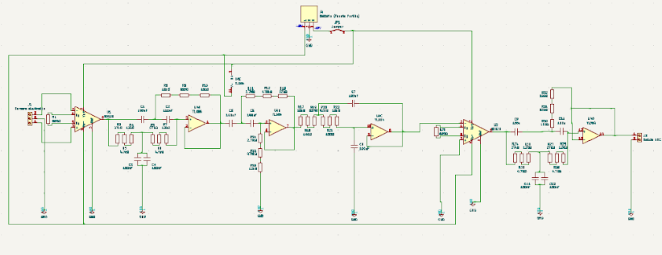
\includegraphics[width=1\linewidth]{Images/Filtros/filtroseeg.png}
    \caption{Esquemático de los filtros del EEG}
\end{figure}

\subsubsection{Esquemático del sistema de control}
\begin{figure}[H]
    \centering
    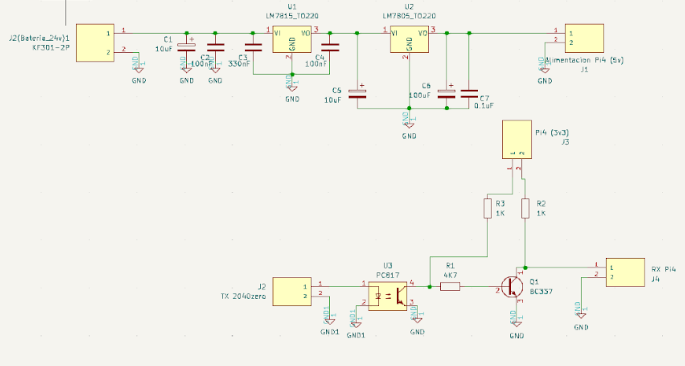
\includegraphics[width=1\linewidth]{Images/SistemaControl/sistemadecontrol.png}
    \caption{Esquemáticos del sistema de control}
\end{figure}

\subsubsection{Esquemático del sistema Offset}
\begin{figure}[H]
    \centering
    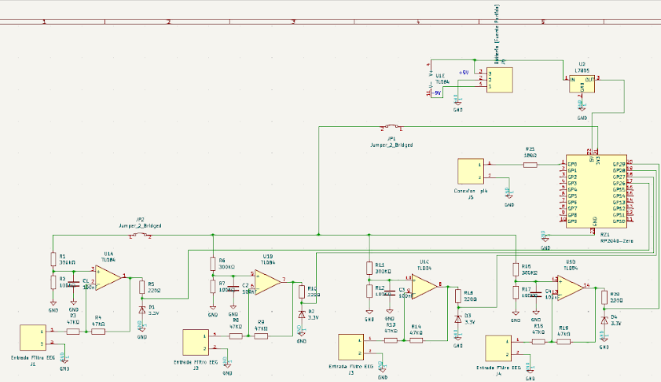
\includegraphics[width=0.95\linewidth]{Images/SistemaOffset/sistemaoffset.png}
    \caption{Esquemático del sistema de Offset}
\end{figure}

\subsubsection{Esquemáticos de los Puentes H}
\begin{figure}[H]
    \centering
     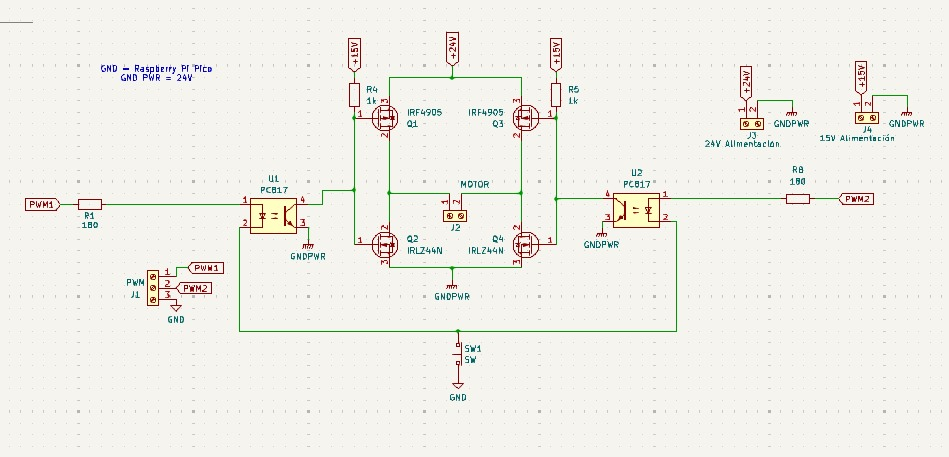
\includegraphics[width=1\textwidth]{Images/PuenteH/WhatsApp Image 2024-08-28 at 9.05.56 AM.jpeg}
    \caption{Puente H (Un Motor)}
\end{figure}

\subsubsection{Esquemático del sistema de emergencia}
\begin{figure}[H]
    \centering
    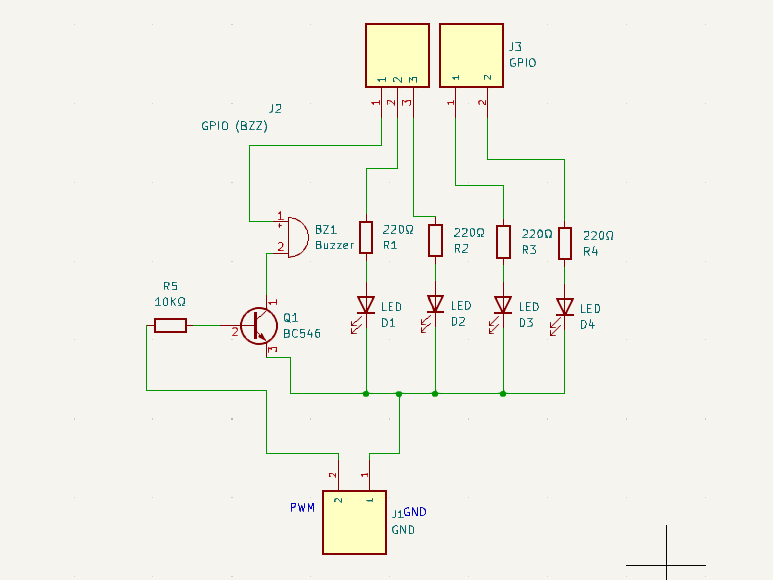
\includegraphics[width=1\textwidth]{Images/SistemaEmergencia/sistemergencia.png}
    \caption{Esquemático del sistema de emegencia}


    \begin{subfigure}[t]{0.5\textwidth}
        \centering
        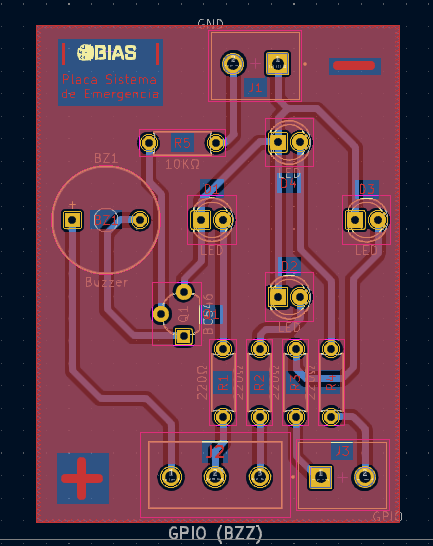
\includegraphics[width=.5\textwidth]{Images/SistemaEmergencia/sistemergenciapcb.png}
        \caption{PCB Del sistema de emergencia}
    \end{subfigure}%
    ~ 
    \begin{subfigure}[t]{0.5\textwidth}
        \centering
        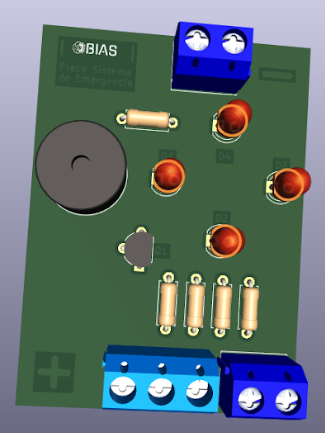
\includegraphics[width=0.5\textwidth]{Images/SistemaEmergencia/sistemergencia3d.png}
        \caption{Modelo 3D Del sistema de emergencia}
    \end{subfigure}

\end{figure}

\subsection{Lista de materiales}
Los programas desarrollados para el proyecto, tales como los filtros digitales, sistemas de inteligencia artificial y otros códigos relacionados, se almacenan en los siguientes dispositivos:

\begin{itemize}
    \item Raspberry Pi 4
    \item RP2040-zero
\end{itemize}

\subsubsection{EEG}
\begin{enumerate}
    \item TL084 (x4)
    \item AD620 (x8)
    \item Capacitores 100nF (x48)
    \item Resistencias 100\Ω (x4)
    \item Resistencias 120\Ω (x16)
    \item Resistencias 560\Ω (x8) 
    \item Resistencias 820\Ω (x16)
    \item Resistencias 1,5k\Ω (x8)
    \item Resistencias 4,7k\Ω (x16)
    \item Resistencias 12k\Ω (x8)
    \item Resistencias 15k\Ω (x8)
    \item Resistencias 27k\Ω (x16)
    \item Resistencias 470k\Ω (x8)
    \item Resistencias 2,7M\Ω (x8)
    \item Electrodos (x9)
\end{enumerate}

\subsubsection{Placa OffSet}
\begin{enumerate}
    \item L7805 (x1)
    \item TL084 (x4)
    \item Jumpers (x2)
    \item Diodos Zenner 3,3V (x4)
    \item Capacitores 100nF (x4)
    \item Resistencias 220\Ω (x4)
    \item Resistencias 50k\Ω (x8)
    \item Resistencias 100k\Ω (x8)
\end{enumerate}

\subsubsection{Sistema de Emergencia}
\begin{enumerate}
    \item Transistor BC546 (x1)
    \item Buzzer 5V (x1)
    \item LEDs Rojos (x4)
    \item Resistencias 220\Ω (x4)
    \item Resistencia 4,7k\Ω (x1)
\end{enumerate}

\subsubsection{Puentes H}
\begin{enumerate}
    \item Transistores IRF4905 (x4)
    \item Transistores IRF2805 (x4)
    \item Optoacopladores PC817 (x4)
    \item Motores 24V 575W (x2)
    \item Resistencias 100\Ω (x4)
    \item Resistencias 180\Ω (x4)
    \item Resistrencias 1k\Ω (x4)
    \item Resistencias 4,7k\Ω (x4)
\end{enumerate}

\subsubsection{Placa reguladora de tensión}
\begin{enumerate}
    \item LM7815 (x1)
    \item Capacitor 100\μF (x1)
    \item Capacitor 330\μF (x1)
    \item Capacitor 470\μF 35V (x1)
    \item Capacitor 470\μF 25V (x1)
\end{enumerate}

\section{Conclusiones}
En esta sección se presentará un análisis detallado de los conocimientos adquiridos a lo largo del desarrollo del proyecto, así como las conclusiones a las que hemos llegado durante este proceso. Se incluirán las conclusiones finales obtenidas, así como una evaluación de las principales limitaciones que afectaron el progreso del trabajo. Además, se ofrecerá un resumen de los resultados alcanzados, destacando los aspectos más relevantes y significativos. Finalmente, se abordarán las perspectivas futuras del proyecto, delineando los pasos a seguir para continuar su desarrollo y mejorarlo en el futuro.


\subsection{Resumen de Resultados}


\subsection{Limitaciones}
Durante la ejecución de este proyecto, nos enfrentamos a diversas limitaciones, algunas de las cuales fueron ocasionadas por circunstancias personales de cada integrante del equipo. Como es común en todo proyecto, al principio experimentamos dificultades en la organización y carecíamos de ciertos conocimientos técnicos, los cuales fuimos adquiriendo a lo largo del año.



El tiempo dedicado al proyecto quizá no fue suficiente, considerando la magnitud y la ambición del mismo. Además de estos desafíos iniciales, una de las principales limitaciones fue el prolongado tiempo de espera para obtener los materiales necesarios, los cuales provenían principalmente de la cooperadora. Dado que esta era nuestra principal fuente de herramientas y componentes, nuestro progreso estuvo estrictamente limitado por los tiempos de adquisición manejados por la institución.


Asimismo, al estar creando algo “nuevo”, nos vimos obligados a adoptar un enfoque basado en la prueba y error, ya que la información disponible sobre los temas específicos que requeríamos era escasa. Esta situación también representó un obstáculo significativo, ya que corregir nuestros errores consumió una parte considerable de nuestro tiempo.


Finalmente, al tratarse de un proyecto desarrollado en el ámbito escolar, también nos vimos limitados por el tiempo disponible en la escuela. No pudimos dedicar todo nuestro tiempo al proyecto, ya que debíamos atender otras asignaturas y compromisos académicos.

\subsection{Trabajo Futuro}
El proyecto presenta un alto potencial de rentabilidad en el futuro, sustentado en su carácter innovador y las posibilidades que ofrece su desarrollo continuo. Al tratarse de un invento único en su categoría, se prevé que, con el tiempo y el trabajo adicional necesario, este dispositivo pueda alcanzar un nivel de madurez suficiente para ser comercializado a gran escala.

La inversión en tiempo y recursos adicionales permitirá perfeccionar sus características técnicas, optimizar su funcionalidad, y adaptar el producto a las necesidades de un mercado en expansión. Una vez finalizado y refinado, el proyecto podrá captar la atención de un público más amplio, lo que incrementará su viabilidad comercial y su posicionamiento en el mercado.

En caso de que el desarrollo del proyecto no se complete en su totalidad, este podrá ser aprovechado por la institución educativa, permitiendo que otros grupos de estudiantes continúen su avance. De esta manera, el proyecto no solo servirá como un recurso valioso para futuras generaciones, sino que también fomentará la colaboración y el aprendizaje continuo dentro de la comunidad académica, garantizando su evolución y finalización.

\subsection {Informacion Adicional}
La silla desarrollada en este proyecto es un prototipo, es decir, puede contener fallas de todo tipo, y es sujeto a modificaciones a futuro. Se recomienda su uso siempre acompañado, en zonas amplias libres de obstáculos. No se debe usar en lugares húmedos o si el equipo está mojado, y la inteligencia artificial está adaptada a las muestras de una persona del equipo del proyecto, por lo que para ser usada por alguien mas se deberán muestrear los patrones de movimiento de esta misma.

\subsubsection{Programas Utilizados}
Para el desarrollo del proyecto, hemos requerido hacer uso de los siguientes porogramas, con sus enlaces principales: \newline


    \href{https://github.com/}{-Github}    
    \newline

    \href{https://code.visualstudio.com/}{-Visual Studio Code}
    \newline

    \href{https://thonny.org/}{-Thonny}
    \newline

    \href{https://es.overleaf.com/project}{-Overleaf}
    \newline

    \href{https://www.jetbrains.com/es-es/pycharm/}{-Pycharm}
    \newline

    \href{https://termius.com/}{-Termius}
    \newline

    \href{https://www.kicad.org/}{-Kicad}
    \newline

    \href{https://livewire.laravel.com/}{-Livewire}
    \newline

    \href{https://www.analog.com/en/resources/design-tools-and-calculators/ltspice-simulator.html}{-LTSpice}
    \newline

    \href{https://github.com/apps/desktop}{-GitHub Desktop}

\subsubsection{Agradecimientos}

Queremos expresar nuestro más profundo agradecimiento a los profesores que nos han brindado su invaluable apoyo en la realización de este proyecto:


Fabrizio Carlassara: Su asistencia fue crucial en la programación de la mayor parte del proyecto, así como en la creación de circuitos y esquemáticos, la búsqueda de materiales y el desarrollo de los filtros necesarios.


Sergio Medina: Nos brindó su experiencia en la presentación y comercialización del proyecto, además de colaborar en la programación, la búsqueda de materiales y la planificación de los puentes H.


Carlos Bianco: Su apoyo fue esencial en las pruebas y acondicionamiento de los motores, proporcionándonos herramientas y baterías para dichas pruebas, además de colaborar en la búsqueda de materiales.


Daniel Espósito: Nos proporcionó motores y materiales, además de enseñarnos a construir los puentes H para los motores y nos ayudó a solucionar problemas con las pistas de los circuitos para las altas corrientes.


Federico Solomiewicz: Colaboró principalmente en el desarrollo de los filtros, proporcionándonos herramientas para el proyecto y estando siempre disponible para resolver cualquier duda que surgiera.


Juan Carlos Ruiz: Su colaboración fue esencial en las pruebas de los motores para la silla de ruedas, además de ayudarnos principalmente en la creación de los puentes H para los motores y sus circuitos impresos.



\section{Referencias}
En este apartado se presentarán de manera detallada las referencias consultadas al inicio del proyecto, las cuales fueron fundamentales para la conceptualización y desarrollo de la idea final. Estas fuentes proporcionaron el marco teórico y práctico necesario para orientar la dirección del trabajo, influyendo en las decisiones tomadas durante el proceso de diseño y ejecución.
\subsubsection{Autodesk Instructables}
A partir de esta página, obtuvimos los primeros circuitos necesarios para el EEG, lo que nos permitió avanzar de manera significativa en el desarrollo del proyecto. Esta fuente de información fue fundamental para sentar las bases técnicas y nos brindó las herramientas necesarias para continuar con el diseño y la implementación del sistema.


\section{Lista de códigos}

\subsection{Códigos principales}

\subsubsection{bias.py}
\lstinputlisting[language=python]{Codigos/CodigosPrincipales/bias.py}

\subsubsection{app.py}

\subsection{Inteligencia artificial}

\subsubsection{bias\_ai.py}

\subsection{Filtrado y procesamiento de señales}

\subsubsection{bias\_dsp.py}

\subsubsection{bias\_graphing.py} 
\lstinputlisting[language=python]{Codigos/Filtrado/bias_graphing.py}

\subsection{Motores}

\subsubsection{bias\_motors.py}
\lstinputlisting[language=python]{Codigos/Motores/bias_motors.py}

\subsection{Recepción de señales}

\subsubsection{bias\_reception.py}
\lstinputlisting[language=python]{Codigos/Recepcion/bias_reception.py}


\subsubsection{CMakeLists.txt}

\subsubsection{pico\_sdk\_import.cmake}

\subsubsection{reception.c}

\subsection{Página Web}
El sitio web ofrece una breve descripción sobre nosotros, nuestros objetivos, y proporciona enlaces a nuestras redes sociales, donde podrán contactarnos o conocer más acerca de nuestro trabajo.

\begin{center}
    \href{https://proyectobias.github.io/Bias/}{Página Web}
\end{center}

\subsubsection{Lenguaje utilizado en la página web y su código}
El desarrollo de la página web se realizó utilizando los lenguajes HTML y CSS.

Aquí se adjuntan los códigos de la página web:

\begin{center}
    Index.css
\end{center}

\lstinputlisting[language=CSS]{PaginaWeb/index.css}

\begin{center}
    Index.html
\end{center}

\lstinputlisting[language=html]{PaginaWeb/index.html}



\end{document}